\section{Shifting Operators}
\frame{\tableofcontents[currentsection]}

\begin{frame}
  \frametitle{Shifting Bits Right}
  \begin{itemize}
    \item \texttt{a >> k} shifts \texttt{a}'s bits \texttt{k} places to the right
    \item \texttt{k} bits "fall off" the cliff at the right
    \item \texttt{k} zeros are added to the left
  \end{itemize}
  \vskip4mm
  \structure{Example}
  \begin{center}
    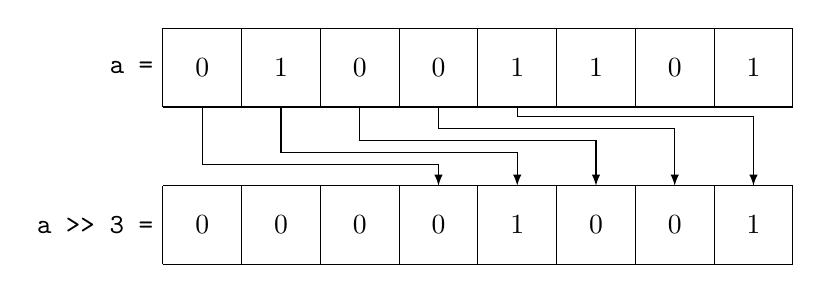
\begin{tikzpicture}
      \draw (0,0) grid (8,1);
      \node[anchor=east,font=\ttfamily] at (0,0.5) {a = };
      \foreach[count=\i,evaluate={\i-0.5} as \x] \v in {0,1,0,0,1,1,0,1} {
        \node at (\x, 0.5) {\v};
      }

      \begin{scope}
        \foreach[count=\i,evaluate={\i-0.5} as \x,evaluate={0.875-\i*0.15} as \y] \v in {1,...,5} {
          \draw[-latex] (\x,0) -- ++(0,-\y) -| (\x+3,-1);
        }
      \end{scope}

      \begin{scope}[yshift=-2cm]
        \draw (0,0) grid (8,1);
        \node[anchor=east,font=\ttfamily] at (0,0.5) {a >> 3 =};
        \foreach[count=\i,evaluate={\i-0.5} as \x] \v in {0,0,0,0,1,0,0,1} {
          \node at (\x, 0.5) {\v};
        }
      \end{scope}
    \end{tikzpicture}
  \end{center}
\end{frame}

\begin{frame}
  \frametitle{Shifting Bits Left}
  \begin{itemize}
    \item \texttt{a << k} shifts \texttt{a}'s bits \texttt{k} places to the left
    \item \texttt{k} bits "fall off" the cliff at the left
    \item \texttt{k} zeros are added to the right
  \end{itemize}
  \vskip4mm
  \structure{Example}
  \begin{center}
    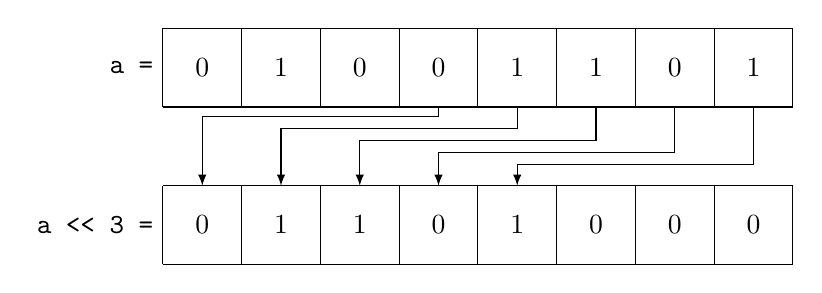
\begin{tikzpicture}
      \draw (0,0) grid (8,1);
      \node[anchor=east,font=\ttfamily] at (0,0.5) {a = };
      \foreach[count=\i,evaluate={\i-0.5} as \x] \v in {0,1,0,0,1,1,0,1} {
        \node at (\x, 0.5) {\v};
      }

      \begin{scope}
        \foreach[count=\i,evaluate={8-\i+0.5} as \x,evaluate={0.875-\i*0.15} as \y] \v in {1,...,5} {
          \draw[-latex] (\x,0) -- ++(0,-\y) -| (\x-3,-1);
        }
      \end{scope}

      \begin{scope}[yshift=-2cm]
        \draw (0,0) grid (8,1);
        \node[anchor=east,font=\ttfamily] at (0,0.5) {a << 3 =};
        \foreach[count=\i,evaluate={\i-0.5} as \x] \v in {0,1,1,0,1,0,0,0} {
          \node at (\x, 0.5) {\v};
        }
      \end{scope}
    \end{tikzpicture}
  \end{center}
\end{frame}
